\documentclass[11pt, letterpaper]{article}
\usepackage{graphicx}
\usepackage{fancybox}
\usepackage[utf8]{inputenc}
\usepackage{epsfig,graphicx}
\usepackage{multicol,pst-plot}
\usepackage{pstricks}
\usepackage{amsmath}
\usepackage{amsfonts}
\usepackage{amssymb}
\usepackage{graphicx}
\usepackage{eucal}
\usepackage{tcolorbox}
\usepackage[czech]{babel}
\usepackage[utf8]{inputenc}
\usepackage[T1]{fontenc}
\usepackage[left=2cm,right=2cm,top=2cm,bottom=2cm]{geometry}
\usepackage{hyperref}
\usepackage{lipsum}
\usepackage{listings}
\usepackage{color}
\usepackage{float}
\setlength{\parindent}{0em}
\setlength{\parskip}{1em}

\lstset{basicstyle=\ttfamily,breaklines=true}

\lstset{extendedchars=\true}
\lstset{inputencoding=ansinew}
\usepackage{xcolor}
\definecolor{codegreen}{rgb}{0,0.6,0}
\definecolor{codegray}{rgb}{0.5,0.5,0.5}
\definecolor{codepurple}{rgb}{0.58,0,0.82}
\definecolor{backcolour}{rgb}{0.95,0.95,0.92}
\lstdefinestyle{mystyle}{
    backgroundcolor=\color{backcolour},   
    commentstyle=\color{codegreen},
    keywordstyle=\color{magenta},
    numberstyle=\tiny\color{codegray},
    stringstyle=\color{codepurple},
    basicstyle=\ttfamily\footnotesize,
    breakatwhitespace=false,         
    breaklines=true,                 
    captionpos=b,                    
    keepspaces=true,                 
    numbers=left,                    
    numbersep=5pt,                  
    showspaces=false,                
    showstringspaces=false,
    showtabs=false,                  
    tabsize=2
}

\lstset{style=mystyle}

\begin{document}
 
\begin{center}
\vfill
{\Huge \textbf{pttypter}}
\vfill
{\huge Uživatelská příručka} \\
{\large verze \texttt{1.0.0}}
\vfill
{\Large Marek Smolík (62880168)} \\
\today
\vfill
\end{center}

\newpage

\section{Úvod}
\texttt{pttypter} je program pro příkazový řádek, který je schopen vzít vstup v podobě syntaktické struktury JSON a následně vrátit tento kód řádně naformátovaný a barevně zvýrazněný. To je schopen provést přímo v příkazovém řádku, nebo jakožto kombinaci HTML a CSS kódu.

\section{Platformová přístupnost}
Program je oficiálně distribuován pro platformy Windows a Linux (x64\_64), avšak v případě Windowsu je minimální podporovaná verze 1909 (ve starších by bylo nutno aktivovat podporu ANSI kódů).

\section{Spouštění}
Jak již bylo řečeno, \texttt{pttypter} je designovaný primárně pro příkazový řádek. Buď \texttt{pttypter} v následujích příkladech cesta k binárnímu programu \texttt{pttypter}. Nápovědu k programu lze vypsat příkazem \texttt{pttypter --h} nebo \texttt{pttypter ----help}.


\begin{figure}[h]
    \begin{center}
        \begin{lstlisting}
$ pttypter -h

pttypter
Marek Smolik, 2022
Simple CLI app to pretty-print JSON

USAGE:
  pttypter [OPTIONS]

FLAGS:
  -h, --help             Prints help information

OPTIONS:
  --input  STRING        The input JSON code
  --theme  STRING        dark/light [DEFAULT: dark]
  --output STRING        html/term  [DEFAULT: term]
        \end{lstlisting}
    \end{center}
    \caption{Výstup po invokaci programu s parametrem \texttt{--h} nebo \texttt{----h}}
\end{figure}

Jediným povinným parametrem je \texttt{----input}, který slouží k zadávání samotného kódu JSON. Parametr \texttt{----theme} slouží k nastavení barevného schéma. Jediné možné hodnoty jsou \texttt{dark} a \texttt{light}. Každá z těchto variant korespenduje k příslušné variaci barevného řežimu inspirovaného stylem \textit{Gruvbox}, původně vytvořeným \href{https://github.com/morhetz}{Pavlem Percevem} pro editor vim. Výchozí hodnota je \texttt{dark}, čiže tmavá varianta.
\begin{figure}[H]
    \begin{center}
        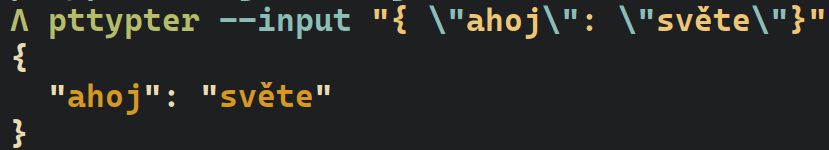
\includegraphics[width=0.8\textwidth]{term}
    \end{center}
    \caption{Ukázka invokace programu se zadáním kódu s výstupem v terminálu}
\end{figure}

Jak lze vidět, program ignoruje všechny whitespace znaky a kód řádně naformátuje a zabarví. Jediným problémem je, že speciální znaky jako \texttt{"} je nutno označit zpětným lomítkem \texttt{\textbackslash}, avšak to je spíše záležitost shellu, kterým je program invokován. 
Uživatelé unixových systémů (respektive uživatelé neprimitivních terminálových prostředí) jistě ocení i možnost použití rour k zadávání vstupu.
\begin{figure}[H]
    \begin{center}
        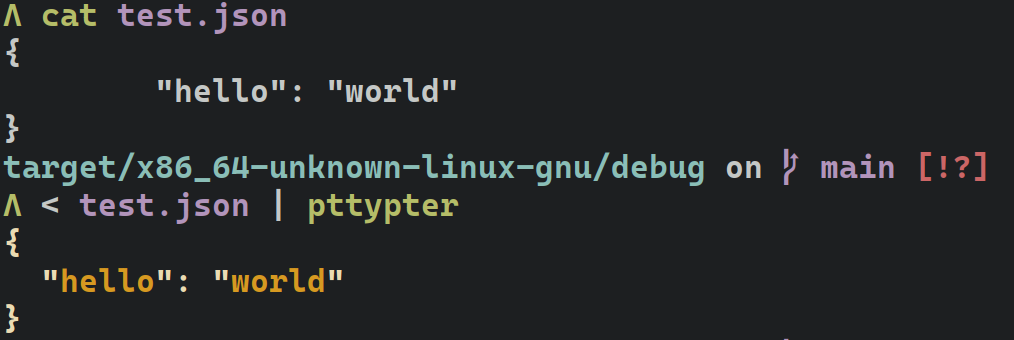
\includegraphics[width=0.8\textwidth]{term2}
    \end{center}
    \caption{Použití rour k zadávání vstupního JSON kódu}
\end{figure}

Druhou, alternativní, možností výstupu je HTML + CSS kód. Ten lze získat například následovně:

\begin{lstlisting}[language=HTML]
$ pttypter --input '{ "je_to_super": True, "problem": null}' --output html --theme light

<style>
		.__pttypter_pre {
			font-family: monospace;
			font-size: inherit;
			display: block;
			background: none;
			white-space: pre;
			-webkit-overflow-scrolling: touch;
			overflow-x: scroll;
			max-width: 100%;
			min-width: 100px;
			padding: 0;
		}

		
		.__pttypter_pre {
			background-color: rgb(251, 241, 199);
			color: rgb(60, 56, 54);
		}

		.__pttypter__fg {
			color: rgb(60, 56, 54);
		}

		.__pttypter__bg {
			color: rgb(251, 241, 199);
		}

		.__pttypter__number {
			color: rgb(177, 98, 134);
		}

		.__pttypter__string {
			color: rgb(215, 153, 33);
		}

		.__pttypter__keyword {
			color: rgb(204, 35, 29);
		}
	
	</style>

	<pre class="__pttypter_pre">
{
&nbsp;&nbsp;"<span class="__pttypter__string">je_to_super</span>": <span class="__pttypter__keyword">True</span>,
&nbsp;&nbsp;"<span class="__pttypter__string">problem</span>": <span class="__pttypter__keyword">null</span>
}
	</pre>

\end{lstlisting}

Někteří z uživatelů opět mohou využít rour a nasměrovat tento výstup programu do nějakého souboru přípony \texttt{html}. Při otevření tohoto souboru (respektive překopírování výstupu) ve webovém prohlížeči lze spatřit blok kódu vygenerovaný programem.

\begin{figure}[H]
    \begin{center}
        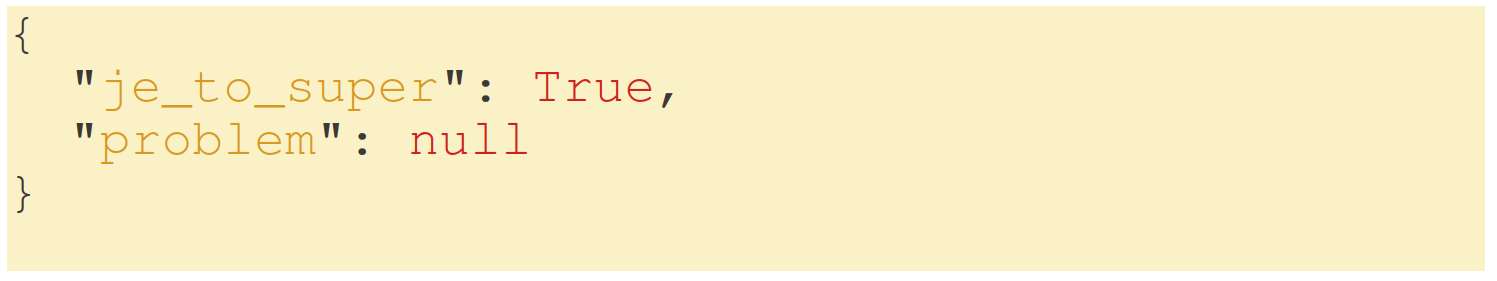
\includegraphics[width=0.8\textwidth]{web1}
    \end{center}
    \caption{Ukázka vyrenderovaného HTML+CSS kódu vygenerovaného \texttt{pttypter}em}
\end{figure}

\section{Validita vstupního kódu}
Program nikdy nevyhodnocuje, zda-li je vstupní kód opravdu validní JSON. Samozřejmě to předpokládá, ale v určitých případech může být záměrně vstupní kód zinvalidněn. V takových případech se program pokusí se vstupem jaksi vypořádat, avšak kvalita výstupu takové procedury není zaručena.

\begin{figure}[H]
    \begin{center}
        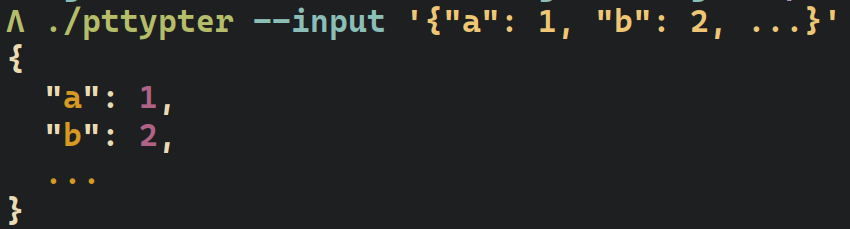
\includegraphics[width=0.8\textwidth]{term3}
    \end{center}
    \caption{Ukázka výstupu programu s invalidním JSON vstupem}
\end{figure}


\end{document}
